
\documentclass[11pt,a4paper,UTF8]{book}

\usepackage[T1]{fontenc}
\usepackage[utf8]{inputenc}
\usepackage{authblk}

\usepackage{ctex} %导入中文包
%\usepackage{ulem}
\usepackage{tocvsec2}

\usepackage{tabularx}
\usepackage{booktabs} 
\usepackage{multirow}
\usepackage{bbding}
\usepackage{float}
\usepackage{xspace}
\usepackage[none]{hyphenat}

\usepackage{graphicx}
\usepackage{subfigure}
\usepackage{pifont}

\usepackage{hyperref}  %制作pdf的目录
\usepackage{subfiles} %使用多文件方式进行

\usepackage{geometry} %设置页边距的包
\geometry{left=2.5cm,right=2cm,top=2.54cm,bottom=2.54cm} %设置书籍的页边距

\usepackage{url}
\hypersetup{hidelinks, %去红框
	colorlinks=true,
	allcolors=black,
	pdfstartview=Fit,
	breaklinks=true
}

% 调整itemlist中的行间距
\usepackage{enumitem}
\setenumerate[1]{itemsep=0pt,partopsep=0pt,parsep=\parskip,topsep=5pt}
\setitemize[1]{itemsep=0pt,partopsep=0pt,parsep=\parskip,topsep=5pt}
\setdescription{itemsep=0pt,partopsep=0pt,parsep=\parskip,topsep=5pt}

% 超链接样式设置
\usepackage{hyperref}
\hypersetup{
	colorlinks=true,
	linkcolor=blue,
	filecolor=blue,
	urlcolor=blue,
	citecolor=cyan,
}

\usepackage{indentfirst}

\usepackage{listings}
\usepackage[usenames,dvipsnames,svgnames, x11names]{xcolor}

\usepackage[most]{tcolorbox}

%展示代码
\definecolor{mygreen}{rgb}{0,0.6,0}
\definecolor{mygray}{rgb}{0.5,0.5,0.5}
\definecolor{mymauve}{rgb}{0.58,0,0.82}
\definecolor{keywordcolor}{rgb}{0.8,0.1,0.5}
\definecolor{webgreen}{rgb}{0,.5,0}
\definecolor{bgcolor}{rgb}{0.92,0.92,0.92}

%定义CMake
\lstdefinelanguage{CMake}
{morekeywords={
		cmake\_minimum\_required,
		project,
		add\_executable,
		add\_library,
		target\_link\_libraries,
		cmake\_parse\_arguments,
		cmake\_language,
		set, unset,
		option,
		string,
		list,
		math,
		message,
		if, elseif, else, endif,
		mark\_as\_advanced,
		foreach, endforeach,
		while, endwhile,
		add\_subdirectory, include, return, include\_gurad,
		function, endfunction,
		macro, endmacro,
		find\_package,
		cmake\_push\_check\_state,
		cmake\_pop\_check\_state,
		cmake\_reset\_check\_state,
		add\_test,
		set\_tests\_properties, 
		check\_c\_source\_runs,
		check\_cxx\_source\_runs,
		check\_fortran\_source\_runs,
		check\_source\_runs,
		check\_compiler\_flag,
		check\_c\_compiler\_flag,
		check\_cxx\_compiler\_flag,
		check\_fortran\_compiler\_flag,
		check\_symbol\_exists,
		check\_cxx\_symbol\_exists,
		check\_linker\_flag,
		cmake\_policy,
		set\_property,
		get\_property,
		define\_property,
		get\_cmake\_property,
		set\_cmake\_property,
		set\_target\_properties,
		get\_target\_property,
		set\_directory\_properties,
		get\_directory\_property,
		set\_source\_files\_properties,
		get\_source\_file\_property,
		set\_tests\_properties,
		get\_tests\_property,
		get\_test\_property,
		cmake\_print\_properties,
		cmake\_print\_variables,
		variable\_watch,
		include\_guard,
		target\_link\_options,
		target\_compile\_definitions,
		target\_compile\_options,
		include\_directories,
		add\_definitions,
		remove\_definitions,
		add\_compile\_definitions,
		add\_compile\_options,
		link\_libraries,
		link\_directories,
		add\_link\_options,
		target\_include\_directories,
		target\_compile\_features,
		add\_custom\_command,
		add\_custom\_target,
		execute\_process,
		cmake\_path,
		get\_filename\_component,
		file,
		configure\_file,
		generate\_export\_header,
		export,
		find\_file,
		find\_library,
		find\_package,
		find\_program,
		pkg\_check\_modules,
		pkg\_search\_module,
		pkg\_get\_variable,
		add\_test,
		enable\_testing,
		set\_tests\_properties,
		site\_name,
		ctest\_empty\_binary\_directory,
		ctest\_start,
		ctest\_configure,
		ctest\_submit,
		ctest\_build,
		ctest\_memcheck,
		ctest\_upload,
		ctest\_test,
		gtest\_add\_tests,
		gtest\_discover\_tests,
		install,
		write\_basic\_package\_version\_file,
		configure\_package\_config\_file,
		cpack\_add\_component,
		cpack\_add\_install\_type,
		cpack\_add\_component\_group,
		ExternalProject\_Add,
		ExternalProject\_Add\_StepDependencies,
		ExternalProject\_Get\_Property,
		ExternalProject\_Add\_Step,
		FetchContent\_Declare,
		FetchContent\_GetProperties,
		FetchContent\_Populate,
		source\_group,
		target\_precompile\_headers,
		qt5\_wrap\_cpp,
		qt5\_wrap\_ui,
		qt5\_add\_resources,
		qt5\_add\_big\_resources,
		qt5\_add\_binary\_resources,
		qt5\_add\_translation,
		qt5\_create\_translation,
		compile\_definitions,
		add\_llvm\_component\_library,
		add\_llvm\_tool,
		llvm\_multisource,
		llvm\_test\_data,
	}, %定义关键字
	sensitive=false, %是否大小写敏感
	morecomment=[l]{\#},
	morestring=[b]",
	morestring=[d]',
}

\lstdefinestyle{styleCMake}{
	language=CMake,
	backgroundcolor=\color{blue!3!white}, 
	basicstyle      =   \zihao{-5}\ttfamily,
	numberstyle     =   \zihao{-5}\ttfamily,
	breakatwhitespace = false,
	breaklines = true,
	captionpos = b,
	commentstyle = \color{mygray}\bfseries, 
	extendedchars =false,             
	frame=shadowbox, 
	tabsize=2,
	framerule=0.5pt,
	keepspaces=true,
	keywordstyle=\color{blue}\bfseries, % keyword style
	otherkeywords={string}, 
	rulecolor=\color{black},
	showspaces=false,
	showstringspaces=false,
	showtabs=false,
	columns         =   fixed,
	stepnumber=1,
	stringstyle=\color{purple},        % string literal style
	flexiblecolumns,  
}


\lstdefinestyle{stylePython}{
	language        =   Python, % 语言选Python
	backgroundcolor=\color{blue!3!white}, 
	basicstyle      =   \zihao{-5}\ttfamily,
	numberstyle     =   \zihao{-5}\ttfamily,
	keywordstyle    =   \color{blue},
	keywordstyle    =   [2] \color{teal},
	stringstyle     =   \color{magenta},
	commentstyle    =   \color{red}\ttfamily,
	frame = shadowbox, 
	breaklines      =   true,   % 自动换行,建议不要写太长的行
	columns         =   fixed,  % 如果不加这一句,字间距就不固定,很丑,必须加
	basewidth       =   0.5em,
	%basicstyle          =   \sffamily,          % 基本代码风格
	%keywordstyle        =   \bfseries,          % 关键字风格
	%commentstyle        =   \rmfamily\itshape,  % 注释的风格,斜体
	%stringstyle         =   \ttfamily,  % 字符串风格
	flexiblecolumns,                % 别问为什么,加上这个
	%numbers             =   left,   % 行号的位置在左边
	showspaces          =   false,  % 是否显示空格,显示了有点乱,所以不现实了
	numberstyle         =   \zihao{-5}\ttfamily,    % 行号的样式,小五号,tt等宽字体
	showstringspaces    =   false,
	captionpos          =   t,      % 这段代码的名字所呈现的位置,t指的是top上面
	frame               =   lrtb,   % 显示边框
	tabsize=2,  
}

\lstdefinestyle{styleCXX}{
	language = C++,  
	backgroundcolor=\color{blue!3!white}, 
	%basicstyle = \footnotesize,  
	basicstyle      =   \zihao{-5}\ttfamily,
	numberstyle     =   \zihao{-5}\ttfamily,   
	%breakatwhitespace = false,    
	basewidth       =   0.5em,    
	breaklines = true,                 
	captionpos = b,                    
	commentstyle = \color{mygreen}\bfseries,
	%extendedchars = false,             
	frame =shadowbox, 
	framerule=0.5pt,
	%frameround = fttt,
	keepspaces=true,
	keywordstyle=\color{blue}\bfseries, % keyword style
	otherkeywords={string}, 
	numbers=left, 
	numbersep=5pt,
	numberstyle=\tiny\color{mygray},
	rulecolor=\color{black},         
	%showspaces=false,  
	%showstringspaces=false, 
	%showtabs=false,    
	%stepnumber=1,         
	stringstyle=\color{mymauve},        % string literal style
	tabsize=2,          
	columns         =   fixed,
	flexiblecolumns,                   
}


\lstdefinelanguage{JavaScript}{
	morekeywords={typeof, new, true, false, catch, function, return, null, catch, switch, var, if, in, while, do, else, case, break, const, console, let},
	morecomment=[s]{/*}{*/},
	morecomment=[l]//,
	morestring=[b]",
	morestring=[b]'
}

\lstdefinestyle{styleJavaScript}{
	language=JavaScript,
	backgroundcolor=\color{blue!3!white}, 
	basicstyle      =   \zihao{-5}\ttfamily,
	numberstyle     =   \zihao{-5}\ttfamily,
	breakatwhitespace = false,
	breaklines = true,
	captionpos = b,
	commentstyle = \color{mygray}\bfseries, 
	extendedchars =false,             
	frame=shadowbox, 
	tabsize=2,
	framerule=0.5pt,
	keepspaces=true,
	keywordstyle=\color{blue}\bfseries, % keyword style
	otherkeywords={string}, 
	rulecolor=\color{black},
	showspaces=false,
	showstringspaces=false,
	showtabs=false,
	columns         =   fixed,
	stepnumber=1,
	stringstyle=\color{purple},        % string literal style
	flexiblecolumns,  
}


\tcbset{
	commandshell/.style={
		listing only,
		colback=black!75!white,
		colupper=white,
		lowerbox=ignored,
		listing options={
			language={bash},
			basicstyle=\ttfamily,
			columns = fixed,
			flexiblecolumns
		}
}}

\usepackage{tikz}

% URL 正确换行
% https://liam.page/2017/05/17/help-the-url-command-from-hyperref-to-break-at-line-wrapping-point/
\makeatletter
\def\UrlAlphabet{%
	\do\a\do\b\do\c\do\d\do\e\do\f\do\g\do\h\do\i\do\j%
	\do\k\do\l\do\m\do\n\do\o\do\p\do\q\do\r\do\s\do\t%
	\do\u\do\v\do\w\do\x\do\y\do\z\do\A\do\B\do\C\do\D%
	\do\E\do\F\do\G\do\H\do\I\do\J\do\K\do\L\do\M\do\N%
	\do\O\do\P\do\Q\do\R\do\S\do\T\do\U\do\V\do\W\do\X%
	\do\Y\do\Z}
\def\UrlDigits{\do\1\do\2\do\3\do\4\do\5\do\6\do\7\do\8\do\9\do\0}
\g@addto@macro{\UrlBreaks}{\UrlOrds}
\g@addto@macro{\UrlBreaks}{\UrlAlphabet}
\g@addto@macro{\UrlBreaks}{\UrlDigits}
\makeatother

% enable subsubsubsection
% from https://tex.stackexchange.com/questions/274212/correct-hierarchy-levels-of-pdf-bookmarks-for-custom-section-subsubsubsection
\usepackage[depth=3]{bookmark}
\setcounter{secnumdepth}{3}
\setcounter{tocdepth}{4}
\hypersetup{bookmarksdepth=4}

\makeatletter

\newcommand{\toclevel@subsubsubsection}{4}
\newcounter{subsubsubsection}[subsubsection]

\renewcommand{\thesubsubsubsection}{\thesubsubsection.\arabic{subsubsubsection}}

\newcommand{\subsubsubsection}{\@startsection{subsubsubsection}{4}{\z@}%
	{-3.25ex\@plus -1ex \@minus -.2ex}%
	{1.5ex \@plus .2ex}%
	{\normalfont\normalsize\bf\bfseries}}

\newcommand*{\l@subsubsubsection}{\@dottedtocline{4}{11em}{5em}}  

\newcommand{\subsubsubsectionmark}[1]{}
\makeatother

\begin{document}
	%\maketitle

	\begin{center}
		\thispagestyle{empty}
		%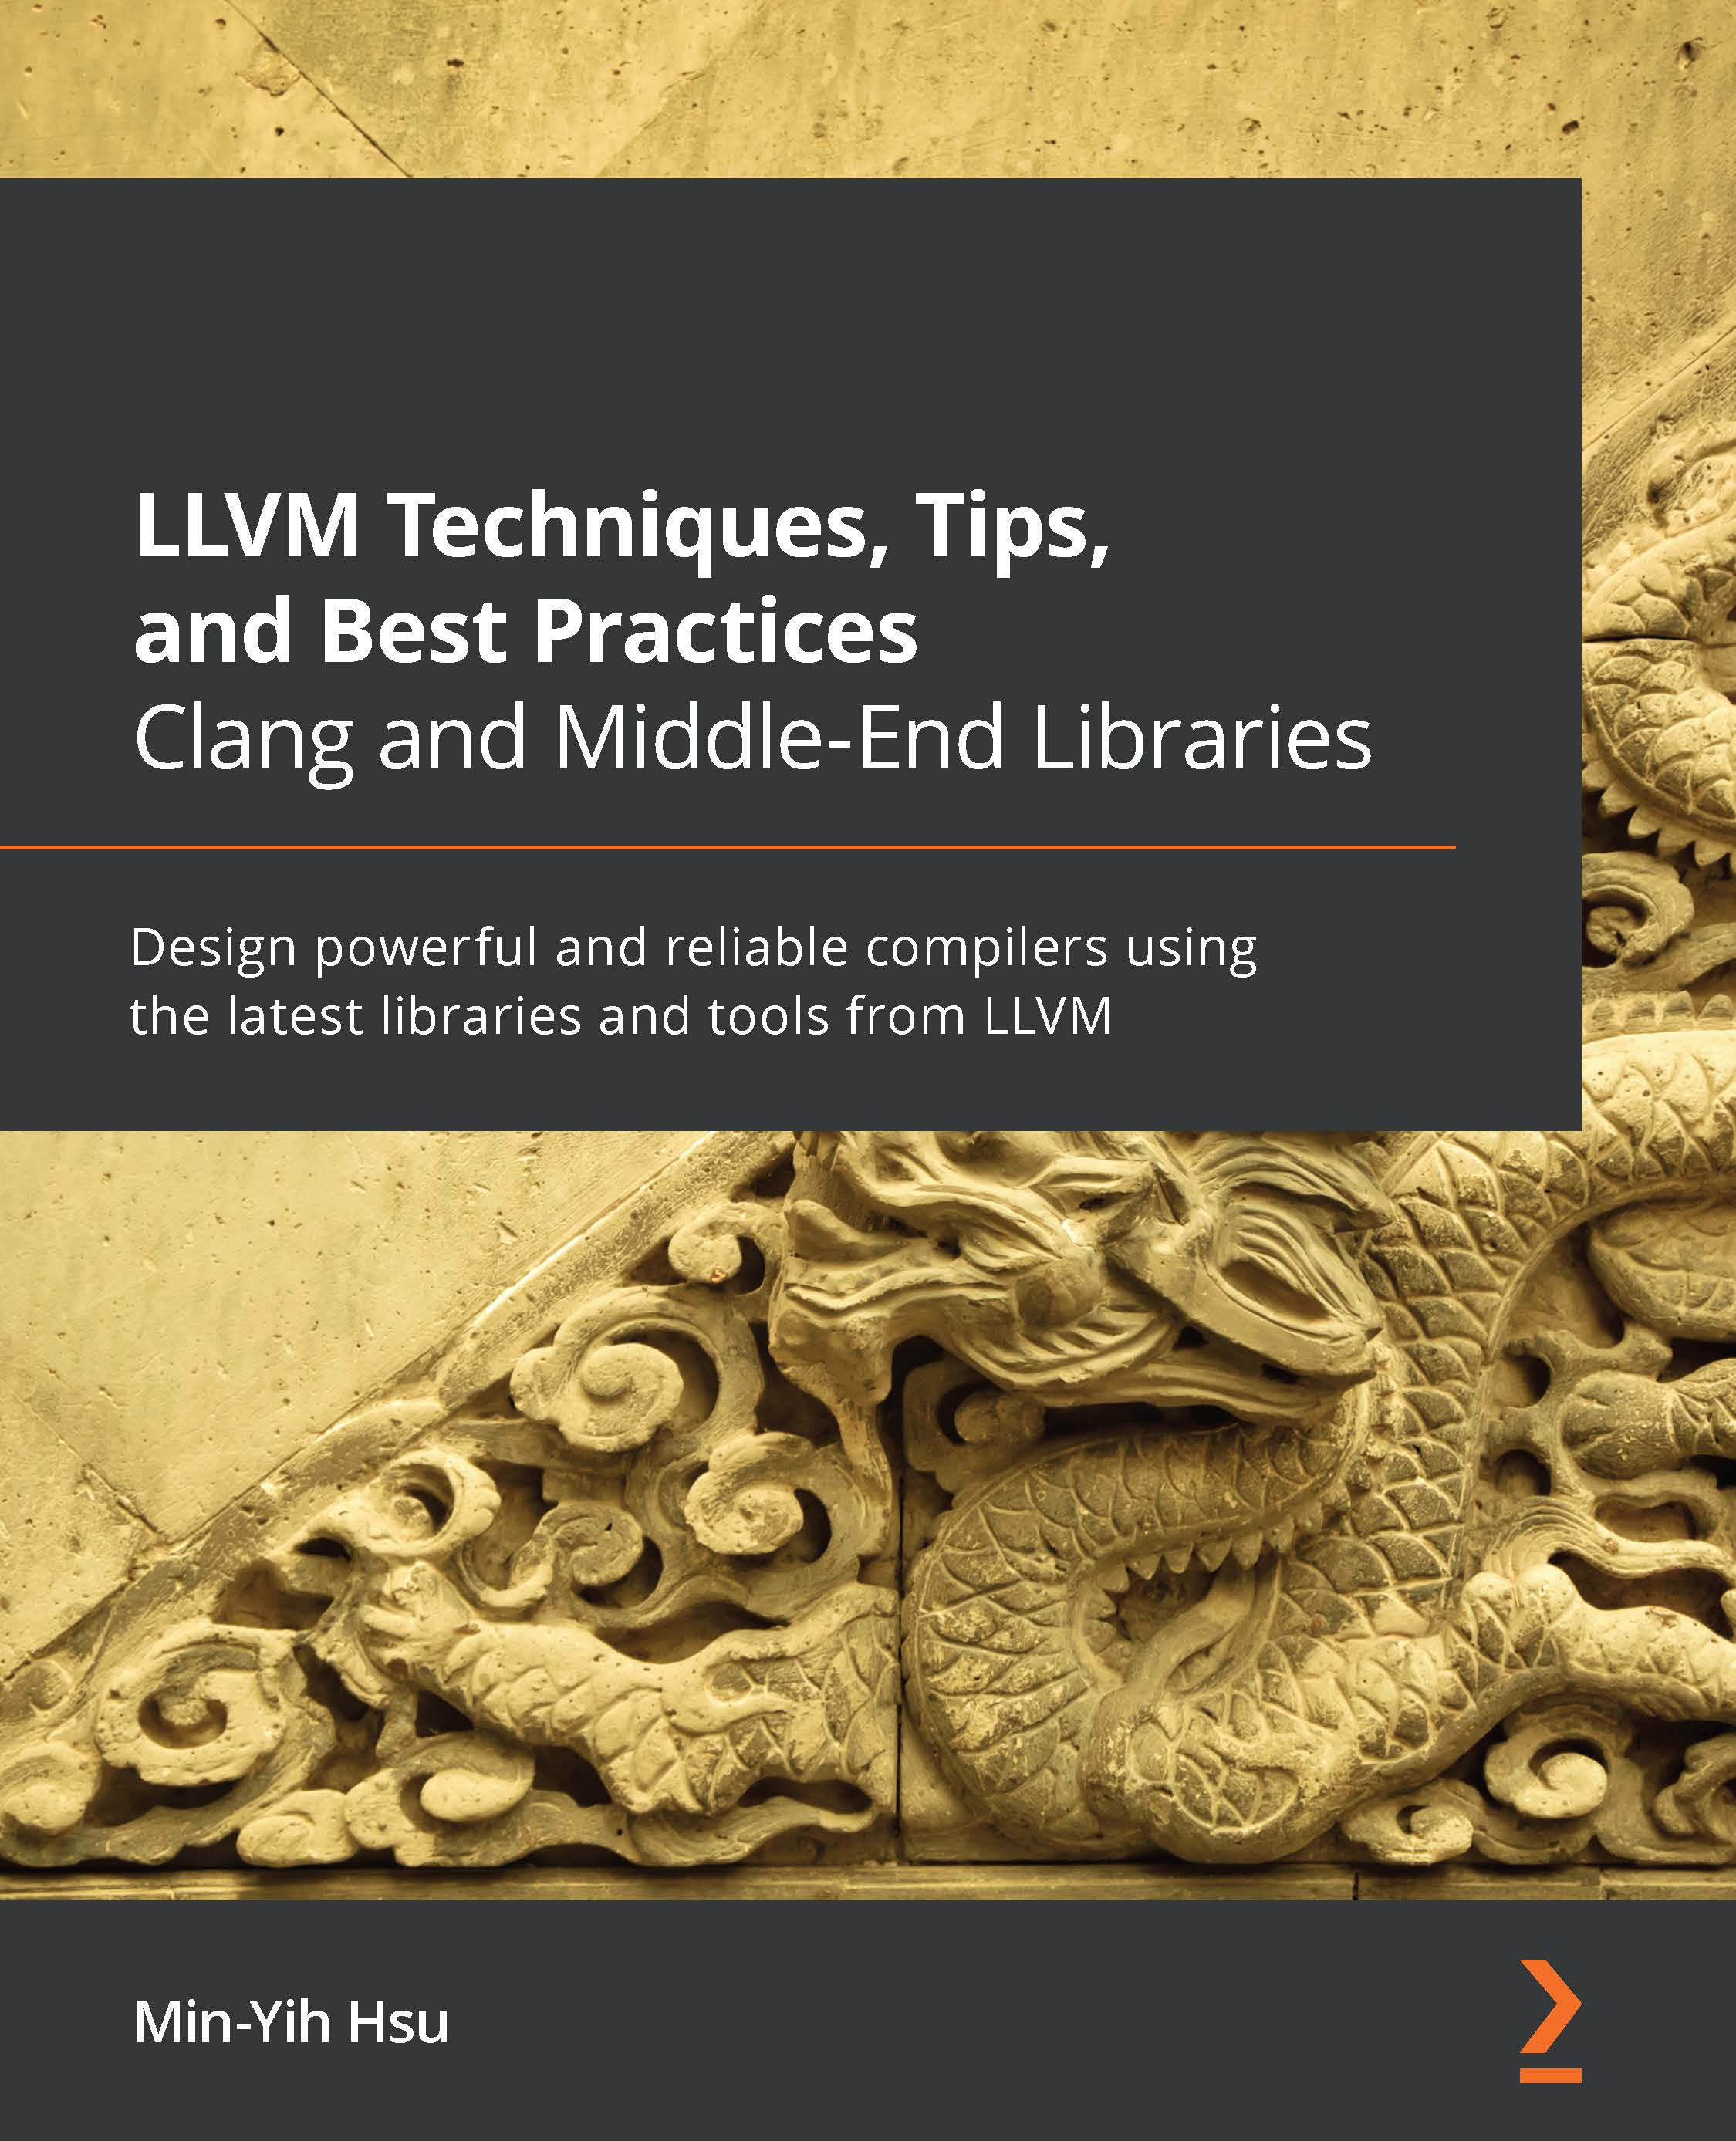
\includegraphics[width=\textwidth,height=\textheight,keepaspectratio]{cover.jpg}
		\begin{tikzpicture}[remember picture, overlay, inner sep=0pt]
			\node at (current page.center) 
			{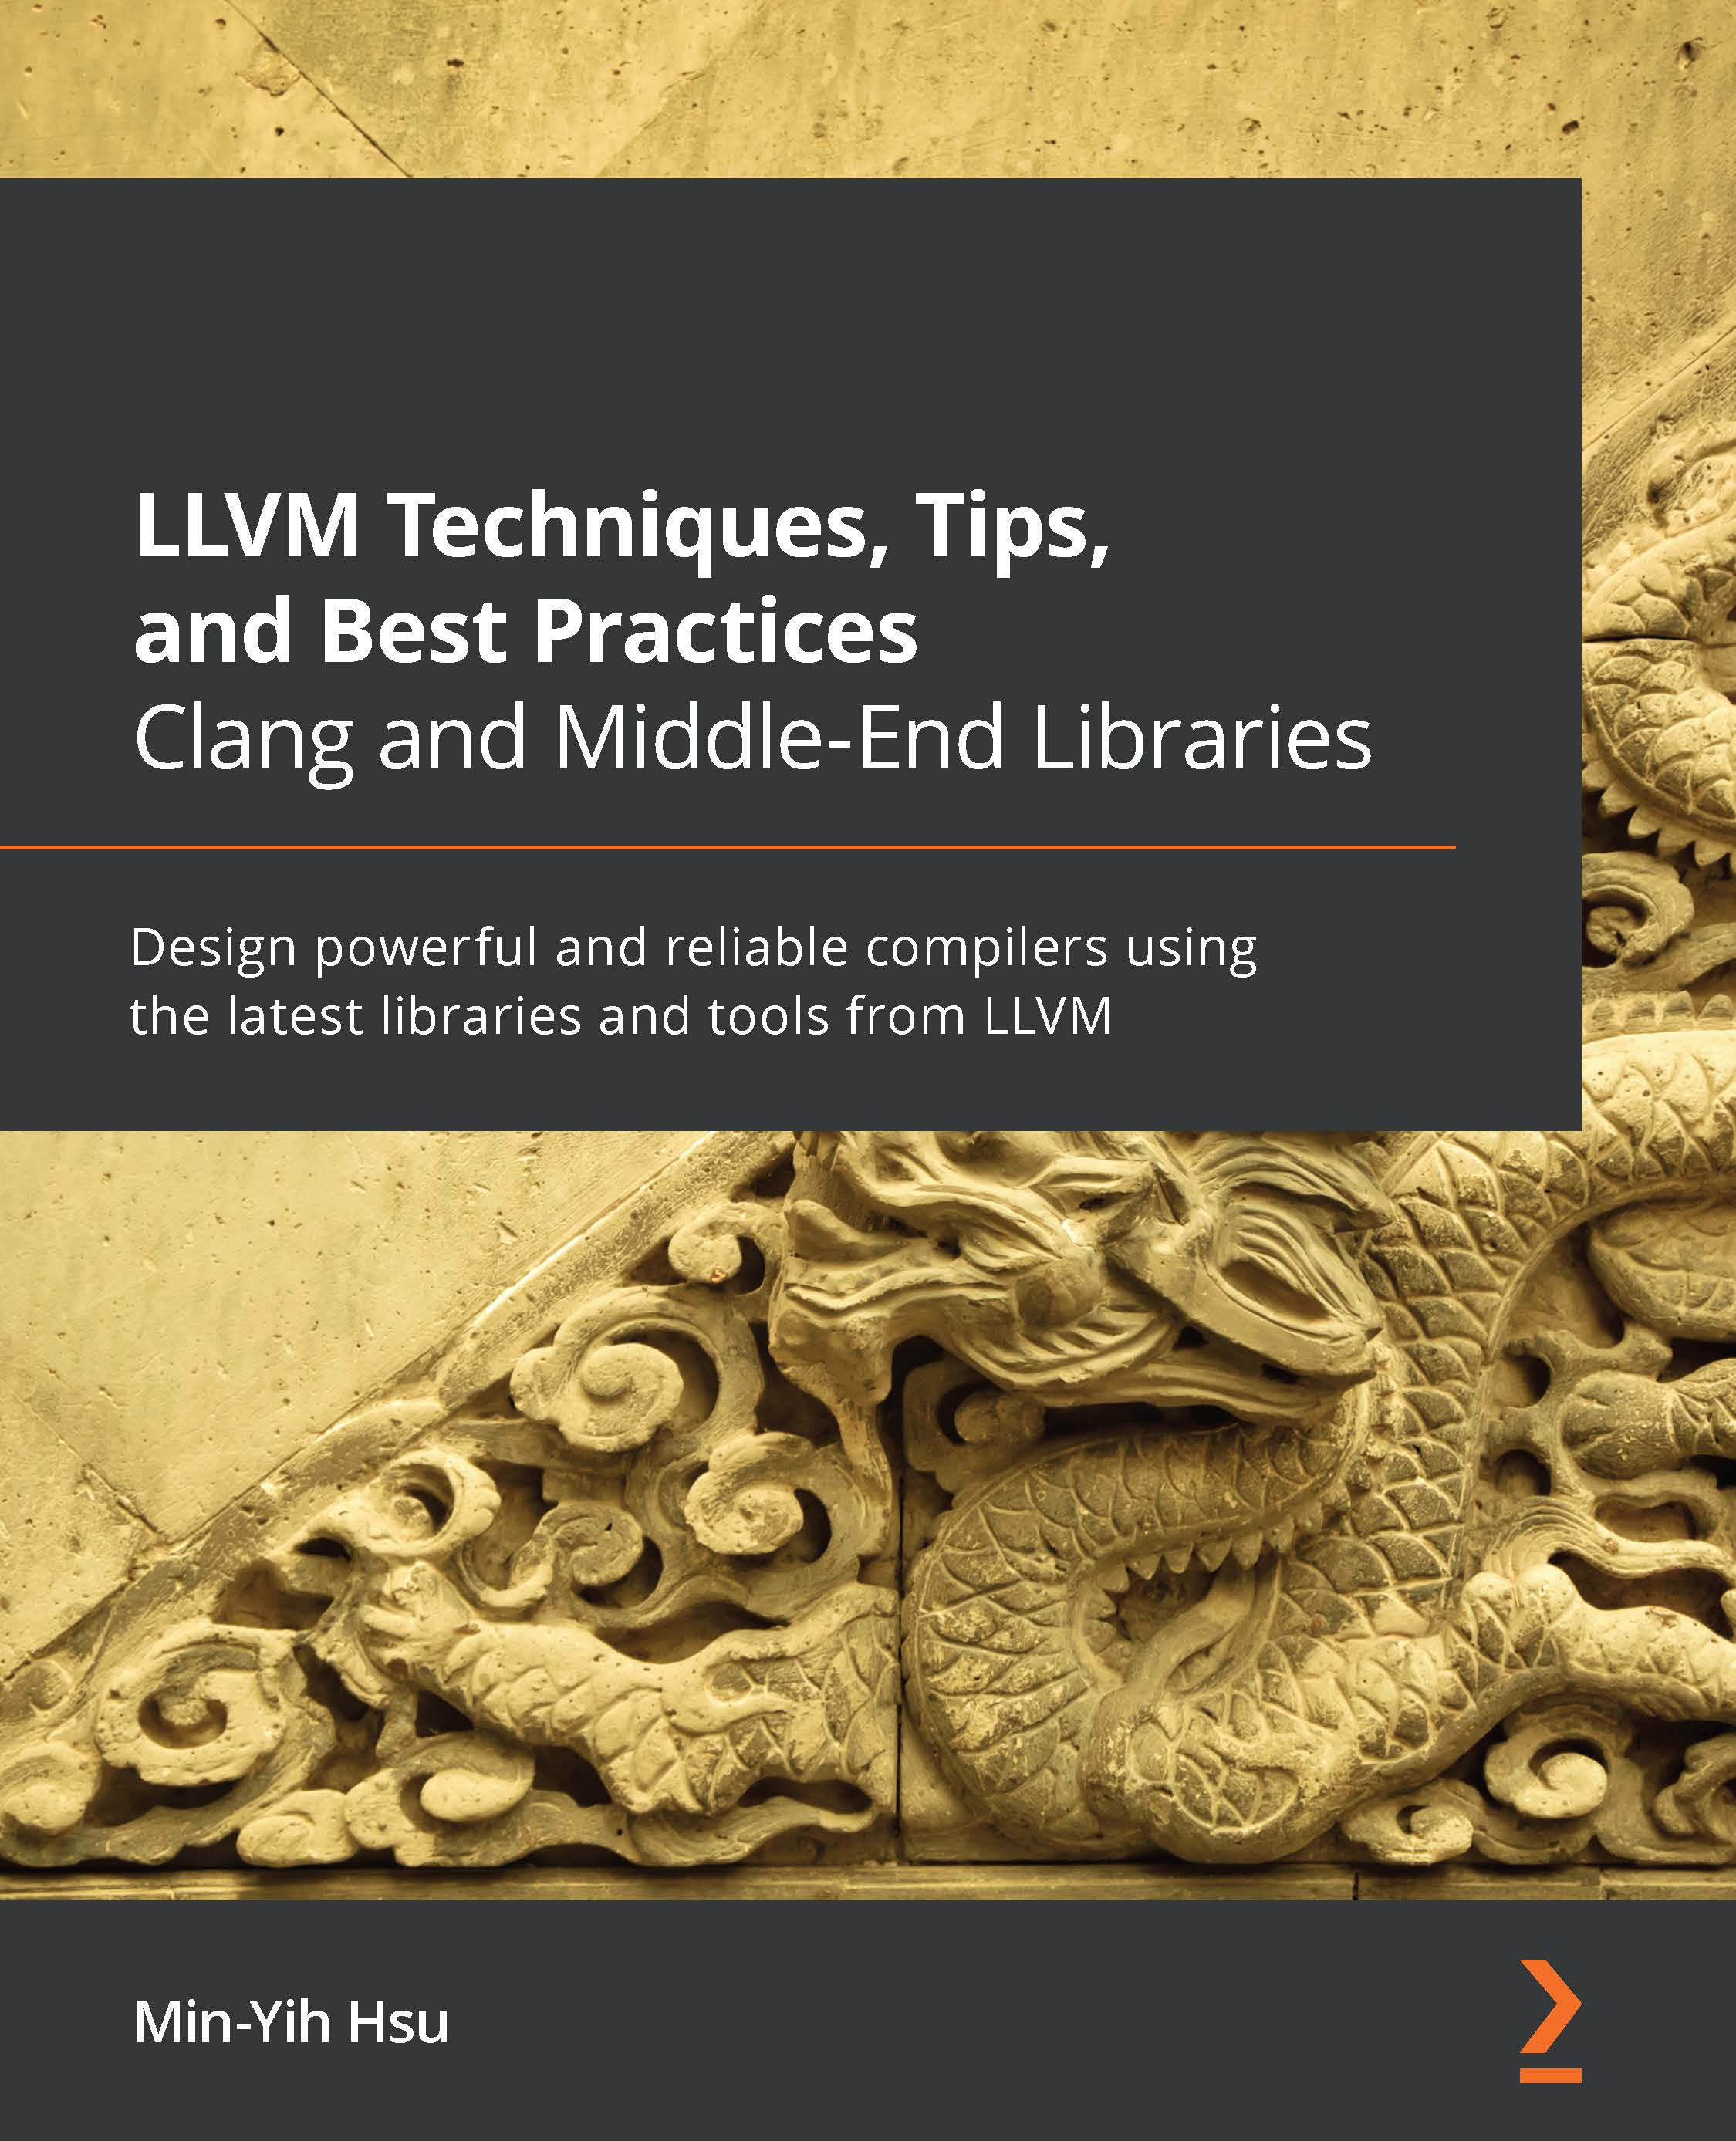
\includegraphics[width=\paperwidth, keepaspectratio=false]{cover.jpg}};
		\end{tikzpicture}
		\newpage
		\thispagestyle{empty}
		\huge
		\textbf{LLVM Techniques, Tips, and Best Practices} 
		\\[9pt]
		\normalsize
		Clang and Middle-End Libraries \\
		Design powerful and reliable compilers using the latest libraries and tools from LLVM \\ 
		(Clang和中端库 - 使用最新的LLVM库和工具设计强大且可靠的编译器)
		\\[10pt]
		\normalsize 
		作者: Min-Yih Hsu 許民易
		\\[8pt]
		\normalsize
		译者;陈晓伟
	\end{center}
	
	\hspace*{\fill} \\ %插入空行
	\noindent\textbf{本书概述}
	
	编译器将高级编程语言转换为低层机器可执行的代码,所以每个程序员或工程师,在职业生涯的某个时刻,都会与编译器一起优化应用程序。LLVM为开发者提供了基础设施、库和(开发人员构建自己的)编译器所需的工具。使用LLVM的工具集,可以有效地为不同的后端生成代码,并进行优化。
	
	本书将探索LLVM编译器的基础结构,并介绍如何来解决问题。我们从查看LLVM重要组件的结构和设计理念开始,逐步使用Clang库来构建分析高级源代码的工具。随着了解的深入,本书将向介绍如何处理LLVM IR——用以转换和优化源码。了解了这些,就将能够利用LLVM和Clang创建编程语言工具,包括编译器、解释器、IDE和源代码分析程序。
	
	本书的最后,可以使用LLVM框架创建强大的工具技能,以应对现实中的各种挑战。
	
	\hspace*{\fill} \\ %插入空行
	\noindent\textbf{关键特性}
	\begin{itemize}
		\item (以务实的方式)探索Clang,LLVM的中端和后端
		\item 点亮LLVM的各个技能点,并掌握各种常见用例
		\item 通过示例应对实际的LLVM开发
	\end{itemize}

	\hspace*{\fill} \\ %插入空行
	\noindent\textbf{内容纲要}
	\begin{itemize}
		\item 了解LLVM的构建系统是如何工作的,以及如何减少构建资源
		\item 掌握使用LLVM的LIT框架运行自定义测试的方法
		\item 为Clang构建不同类型的插件和扩展
		\item 基于Clang自定义工具链和编译器标志
		\item 为PassManager写LLVM Pass
		\item 了解如何检查和修改LLVM IR
		\item 了解如何使用LLVM的配置文件引导优化(PGO)框架
		\item 创建自定义(编译器)消毒器
	\end{itemize}

	本书适用于所有具有LLVM工作经验的软件工程师。如果你是一名学术研究者,这本书将助你在短时间内学习有用的LLVM技能,使你能够快速构建项目原型。编程语言爱好者也会发现这本书中的内容,在LLVM的帮助下构建一种新的编程语言也十分有趣。
	
	\hspace*{\fill} \\ %插入空行
	\noindent\textbf{作者简介}
	
	\textbf{Min-Yih "Min" Hsu}是加州大学欧文分校计算机科学博士研究生。他的研究集中在编译器工程、代码优化、高级硬件架构和系统安全。2015年起,他一直是LLVM社区的活跃成员,并贡献了许多补丁。他还致力于通过各种途径倡导LLVM和编译器工程,比如写博客和发表演讲。在业余时间,他喜欢了解各种不同的咖啡豆和煮咖啡的方法。
	\begin{center}
		\tt
		我要感谢所有支持过我的人,特别是家人和导师。\\还要感谢LLVM社区不论出身的包容和善待每一位成员。
	\end{center}

	\thispagestyle{empty}
	\hspace*{\fill} \\ %插入空行
	\noindent\textbf{审评者介绍}
	
	Suyog Sarda是一名专业的软件工程师和开源爱好者,专注于编译器开发和编译器工具,是LLVM开源社区的积极贡献者。他毕业于了印度浦那工程学院,具有计算机技术学士学位。Suyog还参与了ARM和X86架构的代码性能改进,一直是Tizen项目编译团队的一员,对编译器开发的兴趣在于代码优化和向量化。之前,他写过一本关于LLVM的书,名为《LLVM Cookbook》,由Packt出版。除了编译器,Suyog还对Linux内核开发感兴趣。他在迪拜Birla Institute of Technology的2012年IEEE Proceedings of the International Conference on Cloud Computing, Technologies, Applications, and Management上发表了一篇题为《VM pin and Page Coloring Secure Co-resident Virtualization in Multicore Systems》的技术论文。
	
	他在浦那工程学院获得了技术学士学位。到目前为止,他的工作主要与编译器有关,并他对编译器的性能方面特别感兴趣。他曾致力于DSP图像处理语言的研究,使用LLVM的模块化特性可以根据编译器的需求快速实现。然而,LLVM的文档比较分散,他希望这本书可以为LLVM编译器基础架构提供一种综合性的概述。
	
	
	\hspace*{\fill} \\ %插入空行
	\noindent\textbf{本书相关}
	\begin{itemize}
		\item Github翻译地址:\\\url{https://github.com/xiaoweiChen/LLVM-Techniques-Tips-and-Best-Practies}
	\end{itemize}
	\newpage
	
	%前言
	\pagestyle{empty}
	\subfile{content/preface.tex}
	\newpage
	
	\tableofcontents
	\newpage
	
	\setsecnumdepth{section}
	
	\color{white}
	\section*{\zihao{1} 第一部分:构建系统和LLVM的工具}
	\pagecolor{mygray}
	\addcontentsline{toc}{section}{第一部分:构建系统和LLVM的工具}
	\textbf{\subfile{content/1/Section-1.tex}}
	\color{black}
	\pagecolor{white}
	
	\subsection*{\zihao{2} 第1章\hspace{0.5cm}使用有限的资源构建LLVM}
	\addcontentsline{toc}{subsection}{第1章\hspace{0.5cm}使用有限的资源构建LLVM}
	\subfile{content/1/chapter1/0.tex}
	
	\subsubsection*{\zihao{3} 1.1.\hspace{0.2cm}相关准备}
	\addcontentsline{toc}{subsubsection}{1.1.\hspace{0.2cm}相关准备}
	\subfile{content/1/chapter1/1.tex}
	
	\subsubsection*{\zihao{3} 1.2.\hspace{0.2cm}使用工具减少构建资源}
	\addcontentsline{toc}{subsubsection}{1.2.\hspace{0.2cm}使用工具减少构建资源}
	\subfile{content/1/chapter1/2.tex}
	
	\subsubsection*{\zihao{3} 1.3.\hspace{0.2cm}调整CMake参数}
	\addcontentsline{toc}{subsubsection}{1.3.\hspace{0.2cm}调整CMake参数}
	\subfile{content/1/chapter1/3.tex}
	
	\subsubsection*{\zihao{3} 1.4.\hspace{0.2cm}使用GN获得更快的周转时间}
	\addcontentsline{toc}{subsubsection}{1.4.\hspace{0.2cm}使用GN获得更快的处理时间}
	\subfile{content/1/chapter1/4.tex}
	
	\subsubsection*{\zihao{3} 1.5.\hspace{0.2cm}总结}
	\addcontentsline{toc}{subsubsection}{1.5.\hspace{0.2cm}总结}
	\subfile{content/1/chapter1/5.tex}
	
	\subsubsection*{\zihao{3} 1.6.\hspace{0.2cm}扩展阅读}
	\addcontentsline{toc}{subsubsection}{1.6.\hspace{0.2cm}扩展阅读}
	\subfile{content/1/chapter1/6.tex}
	\newpage
	
	\subsection*{\zihao{2} 第2章\hspace{0.5cm}探索LLVM的构建系统}
	\addcontentsline{toc}{subsection}{第2章\hspace{0.5cm}探索LLVM的构建系统}
	\subfile{content/1/chapter2/0.tex}
	
	\subsubsection*{\zihao{3} 2.1.\hspace{0.2cm}相关准备}
	\addcontentsline{toc}{subsubsection}{2.1.\hspace{0.2cm}相关准备}
	\subfile{content/1/chapter2/1.tex}
	
	\subsubsection*{\zihao{3} 2.2.\hspace{0.2cm}LLVM的CMake指令表}
	\addcontentsline{toc}{subsubsection}{2.2.\hspace{0.2cm}LLVM的CMake指令表}
	\subfile{content/1/chapter2/2.tex}
	
	\subsubsection*{\zihao{3} 2.3.\hspace{0.2cm}如何使用CMake集成LLVM}
	\addcontentsline{toc}{subsubsection}{2.3.\hspace{0.2cm}如何使用CMake集成LLVM}
	\subfile{content/1/chapter2/3.tex}
	
	\subsubsection*{\zihao{3} 2.4.\hspace{0.2cm}总结}
	\addcontentsline{toc}{subsubsection}{2.4.\hspace{0.2cm}总结}
	\subfile{content/1/chapter2/4.tex}
	\newpage
	
	\subsection*{\zihao{2} 第3章\hspace{0.5cm}LLVM LIT测试}
	\addcontentsline{toc}{subsection}{第3章\hspace{0.5cm}LLVM LIT测试}
	\subfile{content/1/chapter3/0.tex}
	
	\subsubsection*{\zihao{3} 3.1.\hspace{0.2cm}相关准备}
	\addcontentsline{toc}{subsubsection}{3.1.\hspace{0.2cm}相关准备}
	\subfile{content/1/chapter3/1.tex}
	
	\subsubsection*{\zihao{3} 3.2.\hspace{0.2cm}在源码树外项目中使用LIT}
	\addcontentsline{toc}{subsubsection}{3.2.\hspace{0.2cm}在源码树外项目中使用LIT}
	\subfile{content/1/chapter3/2.tex}
	
	\subsubsection*{\zihao{3} 3.3.\hspace{0.2cm}FileCheck技巧}
	\addcontentsline{toc}{subsubsection}{3.3.\hspace{0.2cm}FileCheck技巧}
	\subfile{content/1/chapter3/3.tex}
	
	\subsubsection*{\zihao{3} 3.4.\hspace{0.2cm}探索TestSuite框架}
	\addcontentsline{toc}{subsubsection}{3.4.\hspace{0.2cm}探索TestSuite框架}
	\subfile{content/1/chapter3/4.tex}
	
	\subsubsection*{\zihao{3} 3.5.\hspace{0.2cm}总结}
	\addcontentsline{toc}{subsubsection}{3.5.\hspace{0.2cm}总结}
	\subfile{content/1/chapter3/5.tex}
	
	\subsubsection*{\zihao{3} 3.6.\hspace{0.2cm}扩展阅读}
	\addcontentsline{toc}{subsubsection}{3.6.\hspace{0.2cm}扩展阅读}
	\subfile{content/1/chapter3/6.tex}
	\newpage
	
	\subsection*{\zihao{2} 第4章\hspace{0.5cm}TableGen开发}
	\addcontentsline{toc}{subsection}{第4章\hspace{0.5cm}TableGen开发}
	\subfile{content/1/chapter4/0.tex}
	
	\subsubsection*{\zihao{3} 4.1.\hspace{0.2cm}相关准备}
	\addcontentsline{toc}{subsubsection}{4.1.\hspace{0.2cm}相关准备}
	\subfile{content/1/chapter4/1.tex}
	
	\subsubsection*{\zihao{3} 4.2.\hspace{0.2cm}介绍TableGen语法}
	\addcontentsline{toc}{subsubsection}{4.2.\hspace{0.2cm}介绍TableGen语法}
	\subfile{content/1/chapter4/2.tex}
	
	\subsubsection*{\zihao{3} 4.3.\hspace{0.2cm}用TableGen做甜甜圈}
	\addcontentsline{toc}{subsubsection}{4.3.\hspace{0.2cm}用TableGen做甜甜圈}
	\subfile{content/1/chapter4/3.tex}
	
	\subsubsection*{\zihao{3} 4.4.\hspace{0.2cm}用TableGen后端打印食谱}
	\addcontentsline{toc}{subsubsection}{4.4.\hspace{0.2cm}用TableGen后端打印食谱}
	\subfile{content/1/chapter4/4.tex}
	
	\subsubsection*{\zihao{3} 4.5.\hspace{0.2cm}总结}
	\addcontentsline{toc}{subsubsection}{4.5.\hspace{0.2cm}总结}
	\subfile{content/1/chapter4/5.tex}
	
	\subsubsection*{\zihao{3} 4.6.\hspace{0.2cm}扩展阅读}
	\addcontentsline{toc}{subsubsection}{4.6.\hspace{0.2cm}扩展阅读}
	\subfile{content/1/chapter4/6.tex}
	\newpage
	
	\color{white}
	\section*{\zihao{1} 第二部分:LLVM的前端开发}
	\pagecolor{mygray}
	\addcontentsline{toc}{section}{第二部分:LLVM的前端开发}
	\textbf{
		\subfile{content/2/Section-2.tex}
	}
	\color{black}
	\pagecolor{white}
	
	\subsection*{\zihao{2} 第5章\hspace{0.5cm}探索Clang架构}
	\addcontentsline{toc}{subsection}{第5章\hspace{0.5cm}探索Clang架构}
	\subfile{content/2/chapter5/0.tex}
	
	\subsubsection*{\zihao{3} 5.1.\hspace{0.2cm}相关准备}
	\addcontentsline{toc}{subsubsection}{5.1.\hspace{0.2cm}相关准备}
	\subfile{content/2/chapter5/1.tex}
	
	\subsubsection*{\zihao{3} 5.2.\hspace{0.2cm}了解Clang的子系统及其作用}
	\addcontentsline{toc}{subsubsection}{5.2.\hspace{0.2cm}了解Clang的子系统及其作用}
	\subfile{content/2/chapter5/2.tex}
	
	\subsubsection*{\zihao{3} 5.3.\hspace{0.2cm}探索Clang工具的功能和扩展选项}
	\addcontentsline{toc}{subsubsection}{5.3.\hspace{0.2cm}探索Clang工具的功能和扩展选项}
	\subfile{content/2/chapter5/3.tex}
	
	\subsubsection*{\zihao{3} 5.4.\hspace{0.2cm}总结}
	\addcontentsline{toc}{subsubsection}{5.4.\hspace{0.2cm}总结}
	\subfile{content/2/chapter5/4.tex}
	
	\subsubsection*{\zihao{3} 5.5.\hspace{0.2cm}扩展阅读}
	\addcontentsline{toc}{subsubsection}{5.5.\hspace{0.2cm}扩展阅读}
	\subfile{content/2/chapter5/5.tex}
	\newpage
	
	\subsection*{\zihao{2} 第6章\hspace{0.5cm}扩展预处理器}
	\addcontentsline{toc}{subsection}{第6章\hspace{0.5cm}扩展预处理器}
	\subfile{content/2/chapter6/0.tex}
	
	\subsubsection*{\zihao{3} 6.1.\hspace{0.2cm}相关准备}
	\addcontentsline{toc}{subsubsection}{6.1.\hspace{0.2cm}相关准备}
	\subfile{content/2/chapter6/1.tex}

	\subsubsection*{\zihao{3} 6.2.\hspace{0.2cm}使用SourceLocation和SourceManager}
	\addcontentsline{toc}{subsubsection}{6.2.\hspace{0.2cm}使用SourceLocation和SourceManager}
	\subfile{content/2/chapter6/2.tex}
	
	\subsubsection*{\zihao{3} 6.3.\hspace{0.2cm}了解预处理器和词法分析器的基本知识}
	\addcontentsline{toc}{subsubsection}{6.3.\hspace{0.2cm}解预处理器和词法分析器的基本知识}
	\subfile{content/2/chapter6/3.tex}
	
	\subsubsection*{\zihao{3} 6.4.\hspace{0.2cm}定制开发预处理器的插件和回调}
	\addcontentsline{toc}{subsubsection}{6.4.\hspace{0.2cm}定制开发预处理器的插件和回调}
	\subfile{content/2/chapter6/4.tex}
	
	\subsubsection*{\zihao{3} 6.5.\hspace{0.2cm}总结}
	\addcontentsline{toc}{subsubsection}{6.5.\hspace{0.2cm}总结}
	\subfile{content/2/chapter6/5.tex}
	
	\subsubsection*{\zihao{3} 6.6.\hspace{0.2cm}练习}
	\addcontentsline{toc}{subsubsection}{6.6.\hspace{0.2cm}练习}
	\subfile{content/2/chapter6/6.tex}
	\newpage
	
	\subsection*{\zihao{2} 第7章\hspace{0.5cm}处理AST}
	\addcontentsline{toc}{subsection}{第7章\hspace{0.5cm}处理AST}
	\subfile{content/2/chapter7/0.tex}
	
	\subsubsection*{\zihao{3} 7.1.\hspace{0.2cm}Technical requirements}
	\addcontentsline{toc}{subsubsection}{7.1.\hspace{0.2cm}Technical requirements}
	\subfile{content/2/chapter7/1.tex}
	
	\subsubsection*{\zihao{3} 7.2.\hspace{0.2cm}Learning about AST in Clang}
	\addcontentsline{toc}{subsubsection}{7.2.\hspace{0.2cm}Learning about AST in Clang}
	\subfile{content/2/chapter7/2.tex}
	
	\subsubsection*{\zihao{3} 7.3.\hspace{0.2cm}Writing AST plugins}
	\addcontentsline{toc}{subsubsection}{7.3.\hspace{0.2cm}Writing AST plugins}
	\subfile{content/2/chapter7/3.tex}
	
	\subsubsection*{\zihao{3} 7.4.\hspace{0.2cm}总结}
	\addcontentsline{toc}{subsubsection}{7.4.\hspace{0.2cm}总结}
	\subfile{content/2/chapter7/4.tex}
	\newpage
	
	\subsection*{\zihao{2} 第8章\hspace{0.5cm}使用编译器标志和工具链}
	\addcontentsline{toc}{subsection}{第8章\hspace{0.5cm}使用编译器标志和工具链}
	\subfile{content/2/chapter8/0.tex}
	
	\subsubsection*{\zihao{3} 8.1.\hspace{0.2cm}Technical requirements}
	\addcontentsline{toc}{subsubsection}{8.1.\hspace{0.2cm}Technical requirements}
	\subfile{content/2/chapter8/1.tex}
	
	\subsubsection*{\zihao{3} 8.2.\hspace{0.2cm}Understanding drivers and toolchains in Clang}
	\addcontentsline{toc}{subsubsection}{8.2.\hspace{0.2cm}Understanding drivers and toolchains in Clang}
	\subfile{content/2/chapter8/2.tex}
	
	\subsubsection*{\zihao{3} 8.3.\hspace{0.2cm}Adding custom driver flags}
	\addcontentsline{toc}{subsubsection}{8.3.\hspace{0.2cm}Adding custom driver flags}
	\subfile{content/2/chapter8/3.tex}
	
	\subsubsection*{\zihao{3} 8.4.\hspace{0.2cm}Adding a custom toolchain}
	\addcontentsline{toc}{subsubsection}{8.4.\hspace{0.2cm}Adding a custom toolchain}
	\subfile{content/2/chapter8/4.tex}
	
	\subsubsection*{\zihao{3} 8.5.\hspace{0.2cm}总结}
	\addcontentsline{toc}{subsubsection}{8.5.\hspace{0.2cm}总结}
	\subfile{content/2/chapter8/5.tex}
	
	\subsubsection*{\zihao{3} 8.6.\hspace{0.2cm}Exercises}
	\addcontentsline{toc}{subsubsection}{8.6.\hspace{0.2cm}Exercises}
	\subfile{content/2/chapter8/6.tex}
	\newpage
	
	\color{white}
	\section*{\zihao{1} 第三部分:LLVM的中端开发}
	\pagecolor{mygray}
	\addcontentsline{toc}{section}{第三部分:LLVM的中端开发}
	\textbf{
		\subfile{content/3/Section-3.tex}
	}
	\color{black}
	\pagecolor{white}
	
	\subsection*{\zihao{2} 第9章\hspace{0.5cm}使用PassManager和AnalysisManager}
	\addcontentsline{toc}{subsection}{第9章\hspace{0.5cm}使用PassManager和AnalysisManager}
	\subfile{content/3/chapter9/0.tex}
	
	\subsubsection*{\zihao{3} 9.1.\hspace{0.2cm}Technical requirements}
	\addcontentsline{toc}{subsubsection}{9.1.\hspace{0.2cm}Technical requirements}
	\subfile{content/3/chapter9/1.tex}
	
	\subsubsection*{\zihao{3} 9.2.\hspace{0.2cm}Writing an LLVM Pass for the new PassManager}
	\addcontentsline{toc}{subsubsection}{9.2.\hspace{0.2cm}Writing an LLVM Pass for the new PassManager}
	\subfile{content/3/chapter9/2.tex}
	
	\subsubsection*{\zihao{3} 9.3.\hspace{0.2cm}Working with the new AnalysisManager}
	\addcontentsline{toc}{subsubsection}{9.3.\hspace{0.2cm}Working with the new AnalysisManager}
	\subfile{content/3/chapter9/3.tex}
	
	\subsubsection*{\zihao{3} 9.4.\hspace{0.2cm}Learning instrumentations in the new PassManager}
	\addcontentsline{toc}{subsubsection}{9.4.\hspace{0.2cm}Learning instrumentations in the new PassManager}
	\subfile{content/3/chapter9/4.tex}
	
	\subsubsection*{\zihao{3} 9.5.\hspace{0.2cm}总结}
	\addcontentsline{toc}{subsubsection}{9.5.\hspace{0.2cm}总结}
	\subfile{content/3/chapter9/5.tex}
	
	\subsubsection*{\zihao{3} 9.6.\hspace{0.2cm}Questions}
	\addcontentsline{toc}{subsubsection}{9.6.\hspace{0.2cm}Questions}
	\subfile{content/3/chapter9/6.tex}
	\newpage
	
	\subsection*{\zihao{2} 第10章\hspace{0.5cm}处理LLVM IR}
	\addcontentsline{toc}{subsection}{第10章\hspace{0.5cm}处理LLVM IR}
	\subfile{content/3/chapter10/0.tex}
	
	\subsubsection*{\zihao{3} 10.1.\hspace{0.2cm}Technical requirements}
	\addcontentsline{toc}{subsubsection}{10.1.\hspace{0.2cm}Technical requirements}
	\subfile{content/3/chapter10/1.tex}
	
	\subsubsection*{\zihao{3} 10.2.\hspace{0.2cm}Learning LLVM IR basics}
	\addcontentsline{toc}{subsubsection}{10.2.\hspace{0.2cm}Learning LLVM IR basics}
	\subfile{content/3/chapter10/2.tex}
	
	\subsubsection*{\zihao{3} 10.3.\hspace{0.2cm}Working with values and instructions}
	\addcontentsline{toc}{subsubsection}{10.3.\hspace{0.2cm}Working with values and instructions}
	\subfile{content/3/chapter10/3.tex}
	
	\subsubsection*{\zihao{3} 10.4.\hspace{0.2cm}Working with loops}
	\addcontentsline{toc}{subsubsection}{10.4.\hspace{0.2cm}Working with loops}
	\subfile{content/3/chapter10/4.tex}
	
	\subsubsection*{\zihao{3} 10.5.\hspace{0.2cm}总结}
	\addcontentsline{toc}{subsubsection}{10.5.\hspace{0.2cm}总结}
	\subfile{content/3/chapter10/5.tex}
	\newpage
	
	\subsection*{\zihao{2} 第11章\hspace{0.5cm}准备相关的工具}
	\addcontentsline{toc}{subsection}{第11章\hspace{0.5cm}准备相关的工具}
	\subfile{content/3/chapter11/0.tex}
	
	\subsubsection*{\zihao{3} 11.1.\hspace{0.2cm}Technical requirements}
	\addcontentsline{toc}{subsubsection}{11.1.\hspace{0.2cm}Technical requirements}
	\subfile{content/3/chapter11/1.tex}
	
	\subsubsection*{\zihao{3} 11.2.\hspace{0.2cm}Printing diagnostic messages}
	\addcontentsline{toc}{subsubsection}{11.2.\hspace{0.2cm}Printing diagnostic messages}
	\subfile{content/3/chapter11/2.tex}
	
	\subsubsection*{\zihao{3} 11.3.\hspace{0.2cm}Collecting statistics}
	\addcontentsline{toc}{subsubsection}{11.3.\hspace{0.2cm}Collecting statistics}
	\subfile{content/3/chapter11/3.tex}
	
	\subsubsection*{\zihao{3} 11.4.\hspace{0.2cm}Adding time measurements}
	\addcontentsline{toc}{subsubsection}{11.4.\hspace{0.2cm}Adding time measurements}
	\subfile{content/3/chapter11/4.tex}
	
	\subsubsection*{\zihao{3} 11.5.\hspace{0.2cm}Error-handling utilities in LLVM}
	\addcontentsline{toc}{subsubsection}{11.5.\hspace{0.2cm}Error-handling utilities in LLVM}
	\subfile{content/3/chapter11/5.tex}
	
	\subsubsection*{\zihao{3} 11.6.\hspace{0.2cm}Learning about the Expected and ErrorOr classes}
	\addcontentsline{toc}{subsubsection}{11.6.\hspace{0.2cm}Learning about the Expected and ErrorOr classes}
	\subfile{content/3/chapter11/6.tex}
	
	\subsubsection*{\zihao{3} 11.7.\hspace{0.2cm}总结}
	\addcontentsline{toc}{subsubsection}{11.7.\hspace{0.2cm}总结}
	\subfile{content/3/chapter11/7.tex}
	\newpage
	
	\subsection*{\zihao{2} 第12章\hspace{0.5cm}学习LLVM IR表达式}
	\addcontentsline{toc}{subsection}{第12章\hspace{0.5cm}学习LLVM IR表达式}
	\subfile{content/3/chapter12/0.tex}
	
	\subsubsection*{\zihao{3} 12.1.\hspace{0.2cm}Technical requirements}
	\addcontentsline{toc}{subsubsection}{12.1.\hspace{0.2cm}Technical requirements}
	\subfile{content/3/chapter12/1.tex}
	
	\subsubsection*{\zihao{3} 12.2.\hspace{0.2cm}Developing a sanitizer}
	\addcontentsline{toc}{subsubsection}{12.2.\hspace{0.2cm}Developing a sanitizer}
	\subfile{content/3/chapter12/2.tex}
	
	\subsubsection*{\zihao{3} 12.3.\hspace{0.2cm}Working with PGO}
	\addcontentsline{toc}{subsubsection}{12.3.\hspace{0.2cm}Working with PGO}
	\subfile{content/3/chapter12/3.tex}
	
	\subsubsection*{\zihao{3} 12.4.\hspace{0.2cm}总结}
	\addcontentsline{toc}{subsubsection}{12.4.\hspace{0.2cm}总结}
	\subfile{content/3/chapter12/4.tex}
	\newpage

	\subsection*{\zihao{2} Assessments}
	\addcontentsline{toc}{subsection}{Assessments}
	\subfile{content/assessments.tex}
	
\end{document}

